\documentclass[a4paper]{article}
\usepackage[utf8]{inputenc}
\usepackage[spanish, es-tabla, es-noshorthands]{babel}
\usepackage[table,xcdraw]{xcolor}
\usepackage[a4paper, footnotesep = 1cm, width=20cm, top=2.5cm, height=25cm, textwidth=18cm, textheight=25cm]{geometry}
%\geometry{showframe}

\usepackage{tikz}
\usepackage{amsmath}
\usepackage{amsfonts}
\usepackage{amssymb}
\usepackage{float}
\usepackage{graphicx}
\usepackage{caption}
\usepackage{subcaption}
\usepackage{multicol}
\usepackage{multirow}
\setlength{\doublerulesep}{\arrayrulewidth}
\usepackage{booktabs}

\usepackage{hyperref}
\hypersetup{
    colorlinks=true,
    linkcolor=blue,
    filecolor=magenta,      
    urlcolor=blue,
    citecolor=blue,    
}

\newcommand{\quotes}[1]{``#1''}
\usepackage{array}
\newcolumntype{C}[1]{>{\centering\let\newline\\\arraybackslash\hspace{0pt}}m{#1}}
\usepackage[american]{circuitikz}
\usetikzlibrary{calc}
\usepackage{fancyhdr}
\usepackage{units} 
\usepackage{svg}

\graphicspath{{../Ejercicio-1/}{../Ejercicio-2/}{../Ejercicio-3/}{../Ejercicio-4/}{../Ejercicio-5/}}
%\svgpath{{../Ejercicio-1/}{../Ejercicio-2/}{../Ejercicio-3/}{../Ejercicio-4/}{../Ejercicio-5/}}

\pagestyle{fancy}
\fancyhf{}
\lhead{22.05 ASSD}
\rhead{Mechoulam, Lambertucci, Rodriguez, Londero}
\rfoot{Página \thepage}

\begin{document}
\subsection{Análisis y construcción del diagrama de tiempos}
Se construyó para el microprocesador M68HC11 el diagrama de tiempos para un ciclo de lectura/escritura, usando como ejemplo la posición de memoria \$2345, la cual está dentro de la hipotética región del mapa de memoria donde se aloja la memoria para la cual se diseñó el decodificador anteriormente.

\begin{figure}[H]
  \centering
  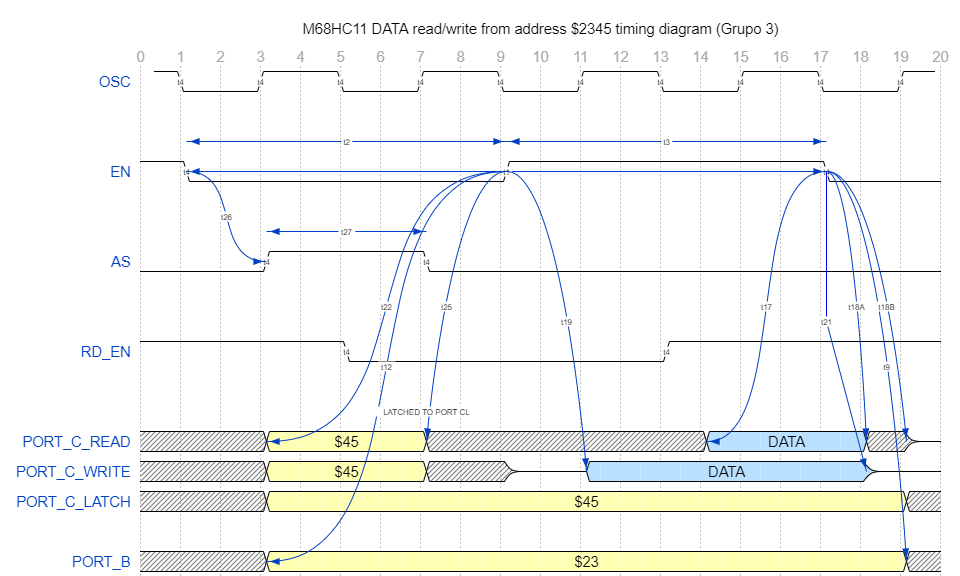
\includegraphics[width=\textwidth]{ImagenesEjercicio1/diagtiempos.png}
  \caption{Ciclo de lectura/escritura de \textit{DATA} en la dirección de memoria \textit{\$2345}}.
  \label{diagtiempos}
\end{figure}
 
Para el análisis de tiempos se tiene en cuenta una frecuencia característica de $2 \ MHz$. Dado esto, se obtiene un rise time de las señales de $t_4 = 20 \ ns$ y un periodo entre ciclos de lectura/escritura de $t_1 = 500 \ ns$, por lo que los tiempos en alto y bajo de la señal \textbf{E} de enable serán de $t_3 = 230 ns$ respectivamente. 

\subsubsection{Primera mitad del ciclo de escritura/lectura}

El comienzo del ciclo de lectura o escritura comienza con el flanco descendente de la señal de enable. Un tiempo $t_{26} = 53 \ ns$ después se activa la señal \textbf{AS} de address strobe, lo cual indica que se utilice el bus de address entero para cargar la parte baja y alta de la dirección de memoria en los puertos C y B del M68HC11 respectivamente. Esta señal se desactiva luego de un tiempo $t_{27} = 96 \ ns$ activando el latch que retendrá la parte baja de la dirección de memoria. De esta manera se logra multiplexar la parte baja del bus de address, o puerto C, para leer o escribir datos al igual que retener la parte baja de la dirección del mapa de memoria.

El puerto C tiene la dirección de memoria por un tiempo válido de $t_{t22} = 88 \ ns$ como mínimo y el puerto B por un tiempo de $t_{12} = 94 \ ns$ como mínimo, que corresponde con el flanco ascendente de la señal de enable y marca la mitad del ciclo de lectura/escritura.

\subsubsection{Segunda mitad del ciclo de escritura/lectura} 
\textbf{Lectura:}
En el caso de la lectura, el tiempo de setup para que el periférico coloque el dato a su salida y lo mantenga estable antes del flanco descendente de la señal de enable es de $t_{17} = 30 \ ns$ y debe ser mantenido estable por $t_{18A} = 10 \ ns$ pasado dicho flanco. Luego pasa a hiZ el puerto C pasados $t_{18B} = 83 \ ns$ de dicho flanco.

\textbf{Escritura:}
Para el caso de la escritura, el puerto C tiene un delay máximo para contener el dato a escribir de $t_{19} = 128 \ ns$ y un tiempo de hold de $t_{21} = 33 \ ns$ como mínimo, por lo cual el tiempo de escritura deberá ser como máximo de $t_{3} + t_{21} - t_{19} = 143 \ ns$.

Finalmente, el address se mantendrá por un tiempo de $t_9$ tras el flanco descendente de la señal de enable, por lo que el tiempo válido de lectura de la dirección de memoria en un ciclo de $t_1 = 500ns$ será de $t_1 - t_{26} + t_{9} = 480 \ ns$.
 
 
 
 
 
 
 
 
 
 
 
 
 
 
 
 
 
 
 
 
 
 
 
 
 
 
 
 
 
 
 
 
%\begin{table}[H]
%\centering
%\begin{tabular}{cccc}
%\hline
%\textbf{A15} & \textbf{A14} & \textbf{A13} & \textbf{CS} \\
%\hline
%0            & 0            & 0            & 0           \\
%0            & 0            & 1            & 0           \\
%\textcolor{red}{0}           & \textcolor{red}{1}            %& \textcolor{red}{0}            & \textcolor{red}{1}           %\\
%\textcolor{red}{0}            & \textcolor{red}{1}            %& \textcolor{red}{1}            & \textcolor{red}{1}           %\\
%1            & 0            & 0            & 0           \\
%1            & 0            & 1            & 0           \\
%1            & 1            & 0            & 0           \\
%1            & 1            & 1            & 0          \\
%\hline
%\end{tabular}
%\end{table}

\end{document}